\begin{figure}[htbp]

\begin{center}
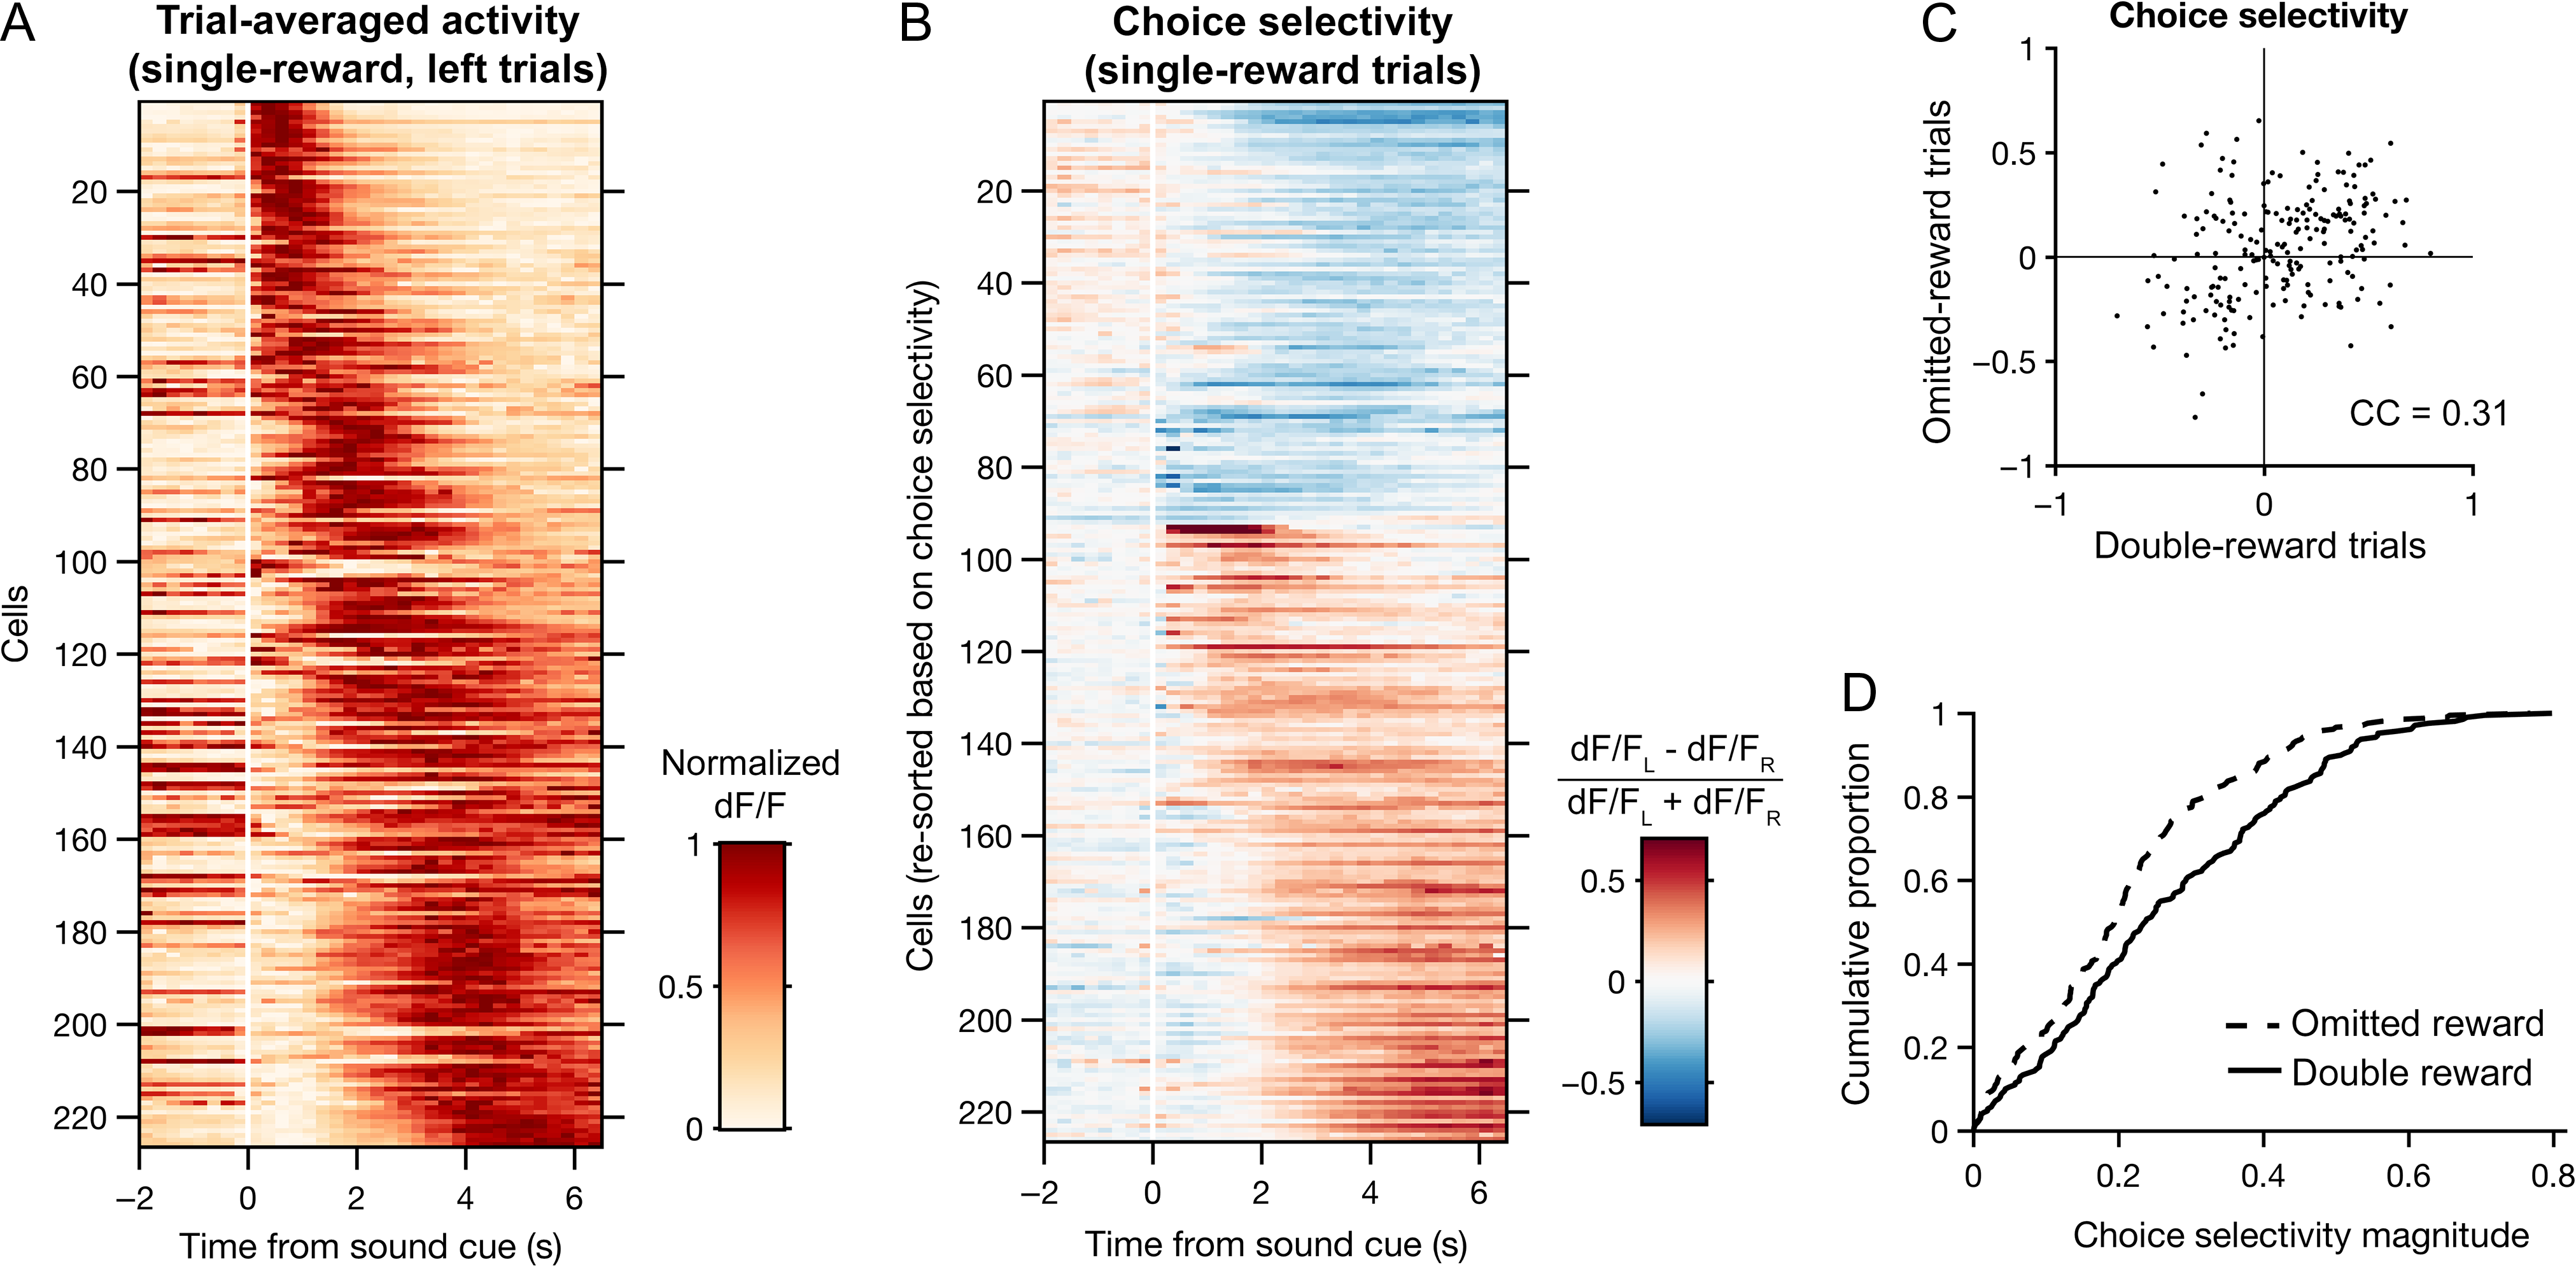
\includegraphics[width=\textwidth]{Figures/CC_fig5.png} 
\end{center}

\caption[Choice representations were modified by trial outcome.]
{Choice representations in M2 are modified by trial outcome. (A) Heat map of trial-averaged fluorescence as a function of time for all choice-selective neurons during single-reward, left trials. Cells are sorted by the center-of-mass of their trial-averaged fluorescence traces. $n = 226$ cells with significant encoding of choice or an interaction of choice and outcome as determined by multiple linear regression (see Methods). (B) Heat map of choice selectivity for the neurons in A as a function of time during single-reward trials. Choice selectivity was calculated as the normalized difference between mean fluorescence traces from left and right trials. Red and blue shadings indicate preference for left and right choices, respectively. Cells are sorted first by mean choice preference and then by the center-of-mass of their choice selectivity traces. (C) Scatter plot of the neurons in A, plotting the choice selectivity of each cell in omitted-reward trials against double-reward trials. $R$, Pearson correlation coefficient. (D) Empirical cumulative distribution of choice selectivity magnitudes for double-reward (solid) and omitted-reward (dotted) trials.}

\label{fig:CC_fig5}
\end{figure}